This section aims to explore concepts that are less widely known among researchers outside the area of regular languages. Along with summarizing the important task of language enumeration algorithms, this section also outlines the backtracking membership algorithm, as well as Glushkov, position, partial derivative, and follow constructions for converting a regular expression into an NFA.


\section{Regular Language Enumeration}
\label{sec:Regular Language Enumeration}
In order to test the efficiency of regular expression membership algorithms, we need to generate words accepted by the regular expression. This is the language enumeration problem, and it can be approached with respect to the regular expression tree as well as an equivalent NFA.

\subsection{Pairwise Word Generation}
\label{subsec:Pairwise Word Generation}
Word generation applied directly onto a regular expression tree is approached as a finite set construction by Zheng et al \cite{pairgen}. One of the main advantages of regular expressions allows the representation of infinite languages using the star operator, so to generate a finite set of words we must limit the number of repetitions allowed of each star. That is, each $(r^*)$ becomes $(r^0 + r^1 + ... + r^k)$ for some integer $1 < k < \infty$. \emph{Combination coverage} is the simplest way to generate words, since we rely on enumerating every word in the language. Its implementation is simple, depending on the structure of each node on the tree. For a regular expression $r$, generate the combination coverage set by calling $C(r)$.

\begin{enumerate}
  \item $C(\alpha \beta) = C(\alpha) C(\beta)$
  \item $C(\alpha + \beta) = C(\alpha) \cup C(\beta)$
  \item $C(\alpha^*) = C(\alpha)^0 \cup C(\alpha)^1 \cup ... \cup C(\alpha)^k$
  \item $C(\alpha?) = \{\epsilon\} \cup C(\alpha)$
  \item $C(\epsilon) = \{\epsilon\}$
  \item $C(\sigma\in\Sigma) = \{\sigma\}$ 
  \item $C( [...\sigma_0-\sigma_1...\sigma_2...]) = ... \cup \{\sigma : \sigma_0 \leq \sigma \leq \sigma_1\} \cup ... \cup \{\sigma_2\} \cup ...$ \\
      (Every symbol accepted by the character class)
\end{enumerate}

However, combination coverage returns an excessive number of words. Not only is this computationally expensive to create (both in time and memory), but a complete set of words is too large when testing an arbitrary regular expression \cite{pairgen}. To limit the number of words, \emph{pairwise} word generation is employed. Pairwise testing applies generally to software where there is a set of variables, each with a finite number of assignments. With combination testing, we test every possible combination of variable assignment. Whereas with pairwise testing we are only concerned with testing pairs of variable assignments \cite{pairwise}. The key idea is to test multiple paired assignments simultaneously.

For the regular expression $r = (a+b)(c+d)(e+f)$, combination coverage enumerates the entire language $|L(r)|=8$. But pairwise coverage is achieved with the set $\{ace, ade, adf, bcf, bde\} \subset L(r)$. This means that every paired combination of assignments is seen in this subset (i.e., $a$ is paired with all $c, d, e, f$; $c$ is paired with all $a,b,e,f$; etc.). Pairwise coverage requires five words, whereas combination coverage requires eight. These savings grow as the regular expression gains complexity.

FAdo implements binary concatenations. This improves simplicity across many algorithms, but totally destroys any savings seen through pairwise concatenation since binary concatenation is pairwise by definition. Instead, we use combination coverage and attempt to limit the number of test cases through problem-specific assumptions:

\begin{enumerate}
  \item $C(.) =$ 16 arbitrarily chosen ASCII symbols
  \item $C([...a-b...c...]) = \{a, b, \sigma, c, ...\}$ for some $\sigma$ between $a,b$
  \item $C(\alpha\beta) =$ no more than 10,000 words sampled randomly (with constant seed) from all possibilities
  \item $C(\alpha^*) = \{\epsilon\} \cup C(\alpha) \cup G$ where $G$ is generated by identifying every pair that needs to be covered, and greedily concatenating them together. We also implemented a hard-limit that helps mitigate against $G$ from containing extremely long words.
    \begin{enumerate}
      \item If $\alpha = (a+b+c)$, which accepts $\{a, b, c\}$, then all \\
          $\{(a,a), (a,b), (a,c), (b,a), (b,b), (b,c), (c,a), (c,b), (c,c)\}$ pairs need to be covered.
      \item Begin arbitrarily with $aa$, then find any pair not yet covered that starts with an $a$. Say, $(a,b)$. The current word being built is now $aab$.
      \item Repeat, but looking for a pair starting with $b$: $(b, a)$. Now the word is $aaba$.
      \item Repeat, but looking for a pair starting with $a$: $(a, c)$. Now the word is $aabac$. \\
            Only the following pairs remain: $\{(b,b), (b,c), (c,a), (c,b), (c,c)\}$.
      \item Continue building the current word until a certain maximum number of repetitions is taken, no more pairs start with the desired letter, or all pairs are used.
      \item Note that in general, letters $a, b, c$ are words of any length.
    \end{enumerate}
\end{enumerate}

\subsection{NFA Language Enumeration}
\label{NFA Language Enumeration}
The other way to enumerate a regular expression $r$ and generate the language $L(r)$ is to construct a sequential NFA $M$ such that $L(M) = L(r)$, and use the  membership algorithm to generate words in lexicographic order. This approach allows a star operation to be maintained as a star operation, instead of having to limit its repetition. 

Consider any sequential NFA construction as the function $A(r)$ (e.g., the Thompson construction with empty-removal construction applied immediately after). The NFA enumeration algorithm describes how to enumerate cross-sections of a given NFA, where the $n^{th}$ cross-section of an NFA is the set of words of length $n$ accepted by the NFA. We use the product construction to construct the acyclic NFA $M_n = A(r) \cap A(.^n)$ where every path from the initial state is of length $n$. First, find the minimal word of $M_n$ by starting at the initial state and greedily taking minimum transitions; concatenate the minimum transition labels, and consider all concatenated words that end in a final state. Given a minimum word $w$, find the next word by running $w$ through the membership algorithm, then backtracking through previous state configurations until the next minimum transition can be taken, then find the minimal word in $M_n$ starting at each potential backtracked state. The entire cross-section has been enumerated when the algorithm backtracks to the initial state from its maximal outgoing transition \cite{nfa-enum}. This process can be repeated for any desired cross-section $n$.





\section{Backtracking Membership Algorithm}
\label{sec:Backtracking Membership Algorithm}
In order for a regular expression implementation to support non-regular operations such as backreferences (as used in some programmer's regular expressions), they must forego typical membership algorithms. Regular languages can decide membership in polynomial time (both using partial derivatives and NFA matching). But after adding non-regular operations such as backreferences, only exponentially bound backtracking algorithms are known. Even using the backtracking algorithm on a mathematical regular expression (i.e., without backreferences) involves an exponential worst-case time complexity. Adding backreferences makes deciding the membership problem NP-complete, since word membership could be solved in (linear) polynomial time to the input word's length if a perfect guessing function was known. Backtracking algorithms consider one state at a time and allow saving additional information like matched groups, whereas regular algorithms consider all possible states at once and rely on collision of these states.

The backtracking membership algorithm can be viewed with respect to a regular expression tree, as well as an NFA \cite{cata-backtrack}. This thesis tests backtracking membership directly using regular expression trees, which avoids the polynomial NFA construction cost. Using generating functions, we are able to write a recursive backtracking algorithm for each type of regular expression node on the regular expression tree. This algorithm tracks the remaining suffix left to match. The $Match$ function returns an iterator of suffixes of the input word. If any substring from the $Match(r, w)$ iterator is empty (i.e., all of $w$ has been matched by $r$), then $r$ accepts $w$. To fit within the scope of the rest of this paper, our implementation of the backtracking algorithm  only supports structures defined in mathematical regular expressions.

\begin{lstlisting}[label={alg:backtracking}, caption={Deciding membership using backtracking}]
Algorithm Backtrack Match($r$, $w$):
    if $r = \alpha\beta$:
        for $s$ in Match($\alpha$, $w$):
            for $s'$ in Match($\beta$, $s$):
                yield $s'$
    else if $r = \alpha|\beta$:
        for $s$ in Match($\alpha$, $w$):
            yield $s$
        for $s$ in Match($\beta$, $w$):
            yield $s$
    else if $r = \alpha^*$:
        for $s$ in Match($\alpha$, $w$):
            for $s'$ in Match($r$, $s$):
                yield $s'$
        yield $w$
    else if $r = \alpha?$:
        for $s$ in Match($\alpha$, $w$):
            yield $s$
        yield $w$
    else if $r = \epsilon$:
        yield $w$
    else if $r = \sigma$ or $r = [...\sigma...]$ or $r = .$:
        yield $\epsilon$
\end{lstlisting}

Algorithm \ref{alg:backtracking} is a modification of Algorithm 1 from \cite{cata-backtrack}, and has been adapted to fit within our mathematical regular expression specification implemented in FAdo. Figure \ref{fig:backtrack_demo}(a) shows the main pitfall of this simple membership algorithm: some words tested on vulnerable regular expressions will experience exponential membership time. In practice, regular expression libraries include many complicated optimizations to limit this exponential cost. Some mitigation strategies include optimizing the regular expression tree to avoid duplicate match options, or using memoization during word evaluation \cite{cata-backtrack, cox}.

\begin{figure}[H]
  \centering
  \begin{subfigure}[b]{0.45\linewidth}
    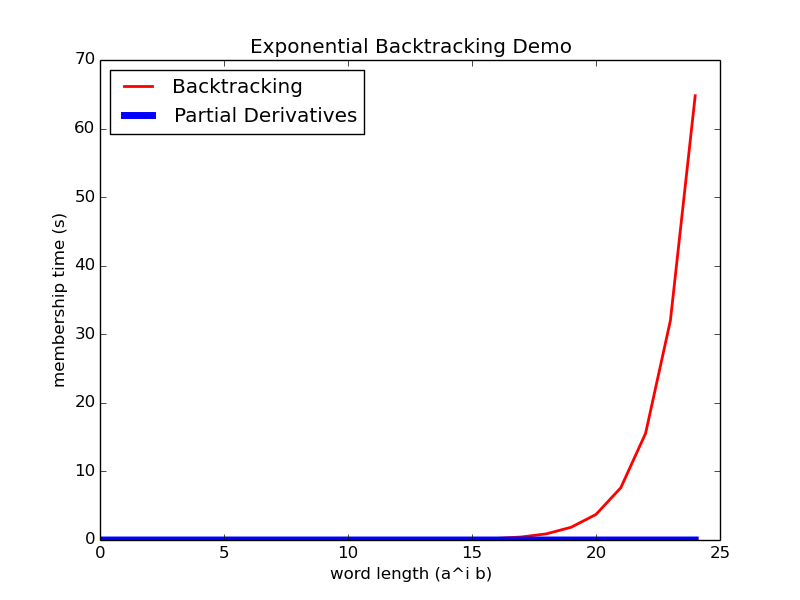
\includegraphics[width=\linewidth]{fig/backtrack_fado}
    \caption{Time to reject words $a^ib$, for $i\in\mathbb{N}$ in $(a+a)^*$ using backtracking vs. partial derivatives.}
  \end{subfigure}
  \hspace{1cm}
  \begin{subfigure}[b]{0.45\linewidth}
    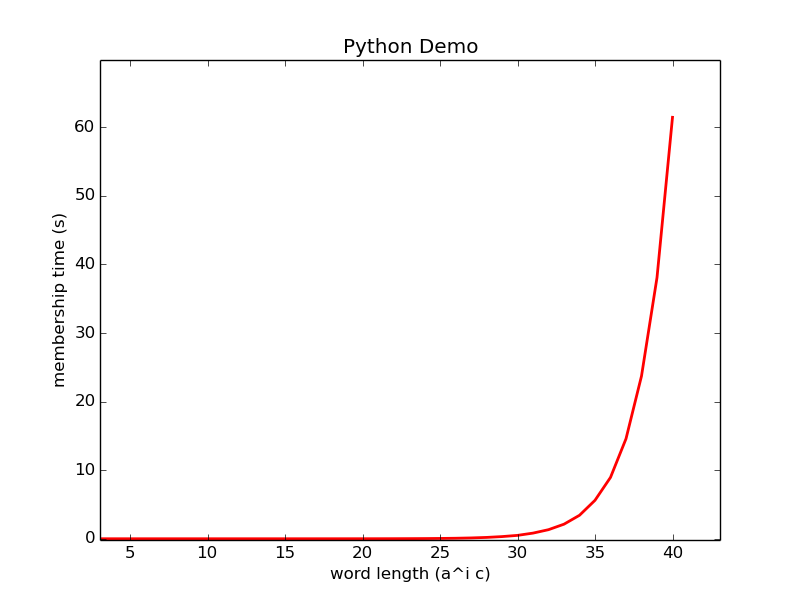
\includegraphics[width=\linewidth]{fig/backtrack_python}
    \caption{Time to reject words $a^ic$, for $i\in\mathbb{N}$ in $(a|aa)^*b$ using Python's built-in re module.}
  \end{subfigure}
  
  \caption{Backtracking suffers from exponential membership time}
  \label{fig:backtrack_demo}
\end{figure}

However, when using a carefully chosen regular expression that avoids structural optimizations, we are able to see exponential growth despite any internal memoization. Figure \ref{fig:backtrack_demo}(b) shows how Python's built-in re module is vulnerable to exponential membership time. This can lead to security vulnerabilities in any application that generates regular expressions based on user input, or uses regular expressions susceptible to a large amount of backtracking (like in Figure \ref{fig:backtrack_demo}). Theoretically, an attacker could launch a backtracking search capable of denying service to other users for hours \cite{cata-backtrack}. Such an attack is referred to as ReDoS (regular expression denial of service).






\section{Glushkov/Position NFA}
\label{sec:Glushkov/Position NFA}
The Glushkov and position constructions are two distinct approaches that build the same NFA. Some authors refer to this NFA as the Glushkov NFA while others call it the position NFA. The Glushkov construction \cite{glushkov-yu} algorithm can be thought of as the Thompson construction without the empty transitions, and potentially with multiple final states. Let states named $p_\alpha$ and $q_\alpha$ be successors of the initial state $i_\alpha$ of a given NFA $\alpha$. For concatenation, each state $f^i_\alpha$ is final if and only if $i_\beta$ is final, then for every transition $(i_\beta, \sigma, p_\beta)$, add transitions $(f^i_\alpha, \sigma, p_\beta)$. Disjunction simply merges the initial states. And star takes a similar approach to concatenation, but without creating any new states and making $i_\alpha$ final. Through every operation, the initial state only has outgoing transitions.

\begin{figure}[H]
  \centering
  \begin{subfigure}[b]{0.22\linewidth}
    \centering
    \begin{tikzpicture}[initial text={}, >={latex}]
      \node[state, initial, accepting] (0) {};
    \end{tikzpicture}
    \caption{Empty word}
  \end{subfigure}
  %
  \begin{subfigure}[b]{0.22\linewidth}
    \centering
    \begin{tikzpicture}[initial text={}, >={latex}]
      \node[state, initial]   (0)                {};
      \node[state, accepting] (1) [right=of 0] {};
      \path[->] (0) edge node [above] {$\sigma$} (1);
    \end{tikzpicture}
    \caption{Atom $\sigma$}
  \end{subfigure}
  %
  \begin{subfigure}[b]{0.45\linewidth}
    \centering
    \begin{tikzpicture}[initial text={}, >={latex}]
      \node[state, initial]   (a0)                      {$i_\alpha$};
      \node[state]            (a1)  [above right=of a0] {$f^1_\alpha$};
      \node[state]            (an)  [below right=of a0] {$f^n_\alpha$};
      \node[draw, fit={(a0)(a1)(an)}]                   {...};      
      \node[state]            (p)   [right=of a1]       {$p_\beta$};
      \node[state]            (q)   [right=of an]       {$q_\beta$};
      \node[state, accepting] (b1)  [right=of p]        {$f^1_\beta$};
      \node[state, accepting] (bn)  [right=of q]        {$f^m_\beta$};
      \node[draw, fit={(p)(q)(b1)(bn)}]                 {...};
      \path[->] (a1) edge [bend left=45, very thick] node [above] {$\sigma_1$} (p)
                (a1) edge [bend left=20, very thick] node [right] {$\sigma_2$} (q)
                (an) edge [bend left=20, very thick] node [left]  {$\sigma_1$} (p)
                (an) edge [bend right=45, very thick] node [below]{$\sigma_2$} (q);
    \end{tikzpicture}
    \caption{Concatenation $(\alpha \beta)$}
  \end{subfigure}
  
  \vspace{1cm}
  
  \begin{subfigure}[b]{0.45\linewidth}
    \centering
    \begin{tikzpicture}[initial text={}, >={latex}]
      \node[state, initial]   (0)                     {$i_\alpha, i_\beta$};
      \node[state, draw=none] (n) [right=of 0]        {};
      \node[state, accepting] (f1) [above right=of n] {$f^1_\alpha$};
      \node[state, accepting] (f2) [above=of f1]      {$f^n_\alpha$};
      \node[state, accepting] (f3) [below right=of n] {$f^1_\beta$};
      \node[state, accepting] (f4) [below=of f3]      {$f^m_\beta$};
      \node[draw, fit={(0)(f1)(f2)}] {... $\alpha$ ...};
      \node[draw, fit={(0)(f3)(f4)}] {... $\beta$ ...};
    \end{tikzpicture}
    \caption{Disjunction $(\alpha + \beta)$}
  \end{subfigure}
  %
  \begin{subfigure}[b]{0.45\linewidth}
    \centering
    \begin{tikzpicture}[initial text={}, >={latex}]
      \node[state, initial, accepting] (0)                     {$i_\alpha$};
      \node[state]            (1) [above right=of 0]  {$p_\alpha$};
      \node[state]            (2) [below right=of 0]  {$q_\alpha$};
      \node[state, accepting] (3) [right=of 1]        {$f^1_\alpha$};
      \node[state, accepting] (4) [right=of 2]        {$f^n_\alpha$};
      \node[draw, fit={(0)(1)(2)(3)(4)}]              {};
      \path[->] (0) edge node [above left] {$\sigma_1$} (1)
                (0) edge node [below left] {$\sigma_j$} (2)
                (3) edge [very thick, bend right=45] node [above] {$\sigma_1$} (1)
                (3) edge [very thick, bend right=20] node [left]  {$\sigma_j$} (2)
                (4) edge [very thick, bend right=20] node [right] {$\sigma_1$} (1)
                (4) edge [very thick, bend left=45]  node [below] {$\sigma_j$} (2);
    \end{tikzpicture}
    \caption{Star $\alpha^*$}
  \end{subfigure}
  \caption{Glushkov construction}
  \label{fig:glushkov construction}
\end{figure}

Although the position automaton \cite{position} is identical to the Glushkov automaton, its construction is significantly different. To convert regular expression $r$ into an NFA using the position construction, we begin by uniquely \emph{marking} each atom in $r$ according to its left-to-right position. For example, the marked version of $a(b+a)b^*$ is $a_1(b_2+a_3)b_4^*$. Then informally define the following functions:

$first(r)$ is the set of marked atoms that could represent the first symbol in a matched word (e.g., $first(a_1(b_2+a_3)b_4^*) = \{a_1\}$). Similarly, $last(r)$ is the set of marked atoms that could represent the last symbol in a matched word (e.g., $last(a_1(b_2+a_3)b_4^*) = \{b_2, a_3, b_4\}$). Finally, $follow(r, \sigma_i)$ is the set of atoms directly reachable in $r$ from the atom $\sigma_i$ (e.g., $follow(a_1(b_2+a_3)b_4^*, b_2) = \{b_4\}$). Because the informal definition is so intuitive, the rigorous approach is not included as it only overcomplicates matters. Curious readers can refer to \cite{follow} for their inductive definitions.

These functions are used in three distinct phases of the position construction. 
First, create an initial state $i$, and for each element $\sigma_i$ in $first(r)$ create the state named $\sigma_i$ if it does not exist, and add transition $(i, \sigma, \sigma_i)$. Mark state $i$ as done.
Then, while there is some state $q_j$ in the NFA not marked as done: iterate through each $\sigma_i \in follow(r, q_j)$. Create the state $\sigma_i$ if it does not exist, and add a transition $(q_j, \sigma, \sigma_i)$ to the NFA, and mark state $\sigma_i$ as done.
Finally, make each state $\sigma_i \in last(r)$ final.





\section{Partial Derivative NFA}
\label{sec:Partial Derivative NFA}
At a high-level, the partial derivative automaton represents all partial derivative possibilities of a regular expression for every alphabet symbol. Each state is named by a regular expression, so the initial state is the original regular expression being encoded, and the final states are any state named $r$ where $\epsilon \in L(r)$. The transition $(p, \sigma, q)$ exists if and only if the set of partial derivatives of $p$ with respect to $\sigma$ includes $q$. That is, $q \in \delta_\sigma(p)$ as defined in Section \ref{sec:Derivatives}.

The approach from Antimirov \cite{Antimirov} defines the \emph{linear form} of a regular expression $p$ as the set of 2-tuples $\{(\sigma, q) : \sigma\in\Sigma, q\in\delta_\sigma(p)\}$. To convert regular expression $r$ into the partial derivative NFA: create a set of newly created states $N$ initialized to $\{r\}$. While there is some newly created state $p$ (representing a regular expression), compute the linear form and iterate through each $(\sigma, q)$ pair. If $q$ has not yet been created, add it to $N$ and create the state. Then for each pair, create the transition $(p, \sigma, q)$.

Because each state of the partial derivative NFA represents a partial derivative derivable from the root $r$ of the regular expression tree, and $pd(r) \leq |r|_\Sigma$, the partial derivative NFA can have no more than $|r|_\Sigma$ states \cite{Antimirov}. This leads to the partial derivative NFA generally having fewer states than other constructions. Additionally, the partial derivative automaton is a quotient of the position automaton; meaning the position automaton can be converted into the partial derivative automaton by merging some states. Figure \ref{fig:nfaPD p tag} illustrates this point with an example using the regular expression accepting HTML paragraph tags. While the partial derivative NFA for this regular expression is of size 13, the Thompson construction creates an NFA of size 50 (omitted due to its large size).

\begin{figure}[H]
  \centering
  \begin{tikzpicture}[initial text={}, >={latex}]
    \node[state, initial]   (0)                     {0};
    \node[state]            (1) [right=of 0]        {1};
    \node[state]            (2) [below right=of 1]  {2};
    \node[state]            (3) [above right=of 2]  {3};
    \node[state, accepting] (4) [right=of 3]        {4};
    \path[->] (0) edge [loop above] node [above]        {$.$}           (0)
              (0) edge              node [above]        {$<$}           (1)
              (1) edge              node [below left]   {/}             (2)
              (1) edge              node [above]        {p}             (3)
              (2) edge              node [below right]  {p}             (3)
              (3) edge [loop above] node [above]        {$[^\wedge >]$} (3)
              (3) edge              node [above]        {$>$}           (4)
              (4) edge [loop above] node [above]        {$.$}           (4);
  \end{tikzpicture}
  \caption{Partial derivative NFA of the expression $.^*(</?p[^\wedge >]>).^*$}
  \label{fig:nfaPD p tag}
\end{figure}

Finding the linear form of a regular expression is costly, especially for large trees. A simple memoization approach lessens the amount of work needed by only computing the linear form for each recursively defined regular expression once, and saving it for future use. This optimized approach is implemented as the ``nfaPDO'' algorithm within FAdo, while the repetitive version is simply ``nfaPD''.

Even when using the optimized construction, the partial derivative automaton was very slow to construct for longer regular expressions until the nfaPDDAG (partial derivative directed acyclic graph) algorithm was published \cite{pddag}. The nfaPDDAG algorithm works by transforming the regular expression tree into a compressed regular expression directed acyclic graph (DAG) without duplicate subtrees; where each node of the compressed regular expression tree is created in the DAG and is uniquely assigned with an increasing index. Each node has no knowledge of the exact regular expression it represents, and instead stores information if the regular expression would have accepted the empty word, and outgoing labelled transitions and their node indices. Once the DAG is constructed, it can be easily converted into an NFA by starting with the root node/index and propagating according to the outgoing labelled transitions.

This algorithm is very fast because it compresses the regular expression (no longer re-computing multiple times for the same subtree in different locations), and uses integer hashing instead of tree hashing. As implemented in FAdo, regular expression tree hashing first converts the tree into a string, then hashes the string using Python's built-in hash function. Tree hashing has a linear cost with the size of the tree, while integer hashing can be done in constant time.





\section{Follow NFA}
\label{sec:Follow NFA}
The follow automaton was first presented by Lucian Ilie and Sheng Yu in 2003 \cite{follow}. In their paper they presented two new automata constructions for regular expression $\alpha$: $A_{follow}^\epsilon(\alpha)$ that constructs an NFA with empty transitions, and $A_{follow}(\alpha)$ that efficiently removes empty transitions from $A_{follow}^\epsilon(\alpha)$. Building $A_{follow}^\epsilon(\alpha)$ for regular expression $\alpha$ is defined inductively, similar to the Thompson construction from Section \ref{sec:Finite Automata}, and is also implemented within FAdo as ``nfaFollowEpsilon'' \cite{fado}.

\begin{figure}[H]
  \centering
  \begin{subfigure}[b]{0.22\linewidth}
    \centering
    \begin{tikzpicture}[initial text={}, >={latex}]
      \node[state, initial, accepting]   (q_0) {};
    \end{tikzpicture}
    \caption{Empty word}
  \end{subfigure}
  %
  \begin{subfigure}[b]{0.22\linewidth}
    \centering
    \begin{tikzpicture}[initial text={}, >={latex}]
      \node[state, initial]   (q_0)                {};
      \node[state, accepting] (q_1) [right=of q_0] {};
      \path[->] (q_0) edge node [above] {$\sigma$} (q_1);
    \end{tikzpicture}
    \caption{Atom $\sigma$}
  \end{subfigure}
  %
  \begin{subfigure}[b]{0.45\linewidth}
    \centering
    \begin{tikzpicture}[initial text={}, >={latex}]
      \node[state, initial]   (q_0)                 {$i_\alpha$};
      \node[state]            (q_1) [right=of q_0]  {$f_\alpha, i_\beta$};
      \node[state, accepting] (q_2) [right=of q_1]  {$f_\beta$};
      \node[draw, fit={(q_0)(q_1)}]                 {...};
      \node[draw, fit={(q_1)(q_2)}]                 {...};
    \end{tikzpicture}
    \caption{Concatenation $(\alpha \beta)$}
  \end{subfigure}
  
  \vspace{1cm}
  
  \begin{subfigure}[b]{0.45\linewidth}
    \centering
    \begin{tikzpicture}[initial text={}, >={latex}]
      \node[state, initial]   (q_0)                      {$i_\alpha, i_\beta$};
      \node[state, draw=none] (qa)  [above right=of q_0] {};
      \node[state, accepting] (q_1) [below right=of qa]  {$f_\alpha, f_\beta$};
      \node[state, draw=none] (qb)  [below right=of q_0] {};
      \node[draw, fit={(q_0)(q_1)(qa)}]                  {};
      \node[draw, fit={(q_0)(q_1)(qb)}]                  {};
      \path[->] (q_0) edge [bend left=75]   node [above] {... $\alpha$ ...} (q_1)
                (q_0) edge [bend right=75]  node [below] {... $\beta$ ...}  (q_1);
    \end{tikzpicture}
    \caption{Disjunction $(\alpha + \beta)$}
  \end{subfigure}
  %
  \begin{subfigure}[b]{0.45\linewidth}
    \centering
    \begin{tikzpicture}[initial text={}, >={latex}]
      \node[state, initial]   (q_0)                 {};
      \node[state]            (q_1) [right=of q_0]  {$i_\alpha, f_\alpha$};
      \node[state, accepting] (q_2) [right=of q_1]  {};
      \node[state, draw=none] (qa)  [above=of q_1]  {};
      \node[draw, fit={(q_1)(qa)}]                  {};
      \path[->] (q_0) edge [very thick] node [above] {$\epsilon$} (q_1)
                (q_1) edge [very thick] node [above] {$\epsilon$} (q_2)
                (q_1) edge [loop above, looseness=15] node [above] {...} (q_1);
    \end{tikzpicture}
    \caption{Star $\alpha^*$}
  \end{subfigure}
  \caption{Follow construction (see below for additional instructions after each step)}
  \label{fig:follow construction}
\end{figure}

For each presented case, a post-processing step is completed to remove unnecessary empty transitions as they are created. 
\begin{itemize}
  \item Concatenation: merge state $f_\alpha, i_\beta$ with any state reachable through one or more \emph{undirected} empty transitions. That is, interpret every $\epsilon$-transition as going both ways.
  \item Star: if $i_\alpha, f_\alpha$ is involved in any cycle with only empty transitions, then all involved states are merged into $i_\alpha, f_\alpha$.
  \item Any case: if the initial state $i$ only has one outgoing transition of the form $(i, \epsilon, i')$, then $i$ is removed and $i'$ becomes the new initial state.
\end{itemize}

This construction is comparable to the Thompson NFA which also uses empty transitions; but the Thompson NFA is always larger. The true follow automaton uses a specialized empty removal construction to return a sequential NFA. The follow NFA is found to be a quotient of the position NFA \cite{follow}.

Although a general case of the empty removal construction is presented in Section \ref{sec:Empty Removal Construction}, the conversion from $A_{follow}^\epsilon(\alpha)$ to the sequential follow NFA $A_{follow}(\alpha)$ is performed in a specific order that improves efficiency. The states $Q$ of $A_{follow}^\epsilon(\alpha)$ are sorted in topological order $Q'$ according to the heuristic:
\begin{center}
  $p, q \in Q: p \leq q \texttt{ iff } (p, \epsilon, q) \in A_{follow}^\epsilon(\alpha).\delta$  
\end{center}
Then, the sorted set of states $Q'$ is considered in reverse order: for each transition $(q \in Q', \epsilon, p)$, find all transitions $(p, \sigma, r)$. Add the transition $(q, \sigma, r)$, remove the transition $(p, \sigma, r)$, and if state $p$ is final, then make $r$ final.

So far, the follow automaton may include disconnected, unreachable, or useless states from the initial state. To \emph{trim} these states, explore through the NFA starting at the initial state and mark any state as useful or not. A state is marked useful if it can be involved in a path from the initial state to any final state. Any unmarked or not useful state is removed along with any of its associated incoming/outgoing transitions. 

\begin{figure}[H]
  \centering
  \begin{subfigure}[b]{0.4\linewidth}
    \centering
    \begin{tikzpicture}[initial text={}, >={latex}]
      \node[state, initial]   (0)                     {0};
      \node[state]            (2) [right=of 0]        {2};
      \node[state]            (3) [below right=of 2]  {3};
      \node[state, accepting] (1) [above right=of 2]  {1};
      \path[->] (0) edge                node [above]      {a, b}       (2)
                (2) edge [loop above]   node [above]      {a, b}       (2)
                (2) edge                node [below right] {$\epsilon$} (1)
                (2) edge [bend left=20] node [above right] {b}         (3)
                (3) edge [loop right]   node [right]       {a}         (3)
                (3) edge [bend left=20] node [below left] {$\epsilon$} (2);
    \end{tikzpicture}
    \caption{$A_{follow}^\epsilon(\alpha)$}
  \end{subfigure}
  %
  \begin{subfigure}[b]{0.4\linewidth}
    \centering
    \begin{tikzpicture}[initial text={}, >={latex}]
      \node[state, initial]   (0)              {0};
      \node[state, accepting] (1) [right=of 0] {1};
      \node[state, accepting] (2) [right=of 1] {2};
      \path[->] (0) edge                node [above]      {a, b}    (1)
                (1) edge [loop above]   node [above]      {a, b}    (1)
                (1) edge [bend left=20] node [above]      {b}       (2)
                (2) edge [bend left=20] node [below]      {a, b}    (1)
                (2) edge [loop above]   node [above]      {a, b}    (2);
    \end{tikzpicture}
    \caption{$A_{follow}(\alpha)$}
  \end{subfigure}
  \caption{Follow construction example \cite{follow}}
  \label{fig:follow construction example}
\end{figure}

Figure \ref{fig:follow construction example} shows an example that illustrates the compactness of the follow automaton (before and after removing empty transitions) for $\alpha = (a+b)(a^*+ba^*+b^*)^*$.



















